\chapter{Umsetzung und Ergebnisse}
\label{cha:umsetzung}
Um die bestmögliche Dokumentation des Systemaufbaus sicherstellen zu können, dürfen die Vorbereitungen, auf die Aufgabe, nicht unterschätzt werden. Diese lassen sich in zwei große Teile aufgeteilen. Der wichtigere von Beiden Schritten ist die sorgfältige Auswahl eines passenden Tools zur Erstellung der Dokumentation. Aspekte wie Benutzerfreundlichkeit, Funktionen die erfüllt werden, Betriebssystemkompatibilitäten und Kosten spielen hier eine große Rolle. Um diese Auswahl mit genügend Sorgfalt zu treffen wird folgendes Vorgehen angewandt:

Es werden verschiedene CAD-Softwareprogramm recherchiert und evaluiert. Die Funktionen stehen hier an erster Stelle. Das Programm muss in der Lage sein, Stromlaufpläne und Bestückungspläne erstellen zu können. An nächster Stelle stehen die Kosten, die für das Programm abgerufen werden. Da das Projekt ein begrenztes Budget hat sollen diese möglichst gering gehalten werden. Wichtig zu beachten ist hierbei jedoch, dass die Kosten im Verhältnis zur gebotenen Leistung des Programms stehen müssen. Die Programme \textit{Autodesk Fusion 360} und \textit{XXX} sind jeweils sehr vielversprechend. 

Nutzerfreundlichkeit gleich
Autodesk für Mac
 Autodesk Fusion 360 kon 
Je nach Art der Arbeit kann diese Kapitelüberschrift auch \glqq Ergebnisse\grqq~lauten, z.~B. bei rein messtechnischen Aufgaben.

Beschreibung der Umsetzung des zuvor gewählten Vorgehens (theoretische Untersuchung, Erhebungen, Durchführung von Experimenten, Prototypenaufbau, Implementierung eines Prozesses, etc.).

Verifikation anhand der zuvor erarbeiteten Anforderungen und Validierung in Bezug auf das zuvor gestellte Ziel. Diskussion der Ergebnisse. Spätestens hier auch auf die Zuverlässigkeit der gewonnenen Erkenntnisse eingehen (z.~B. anhand der Genauigkeit von Messergebnissen).

% Linke Hälfte der A3-Seite
%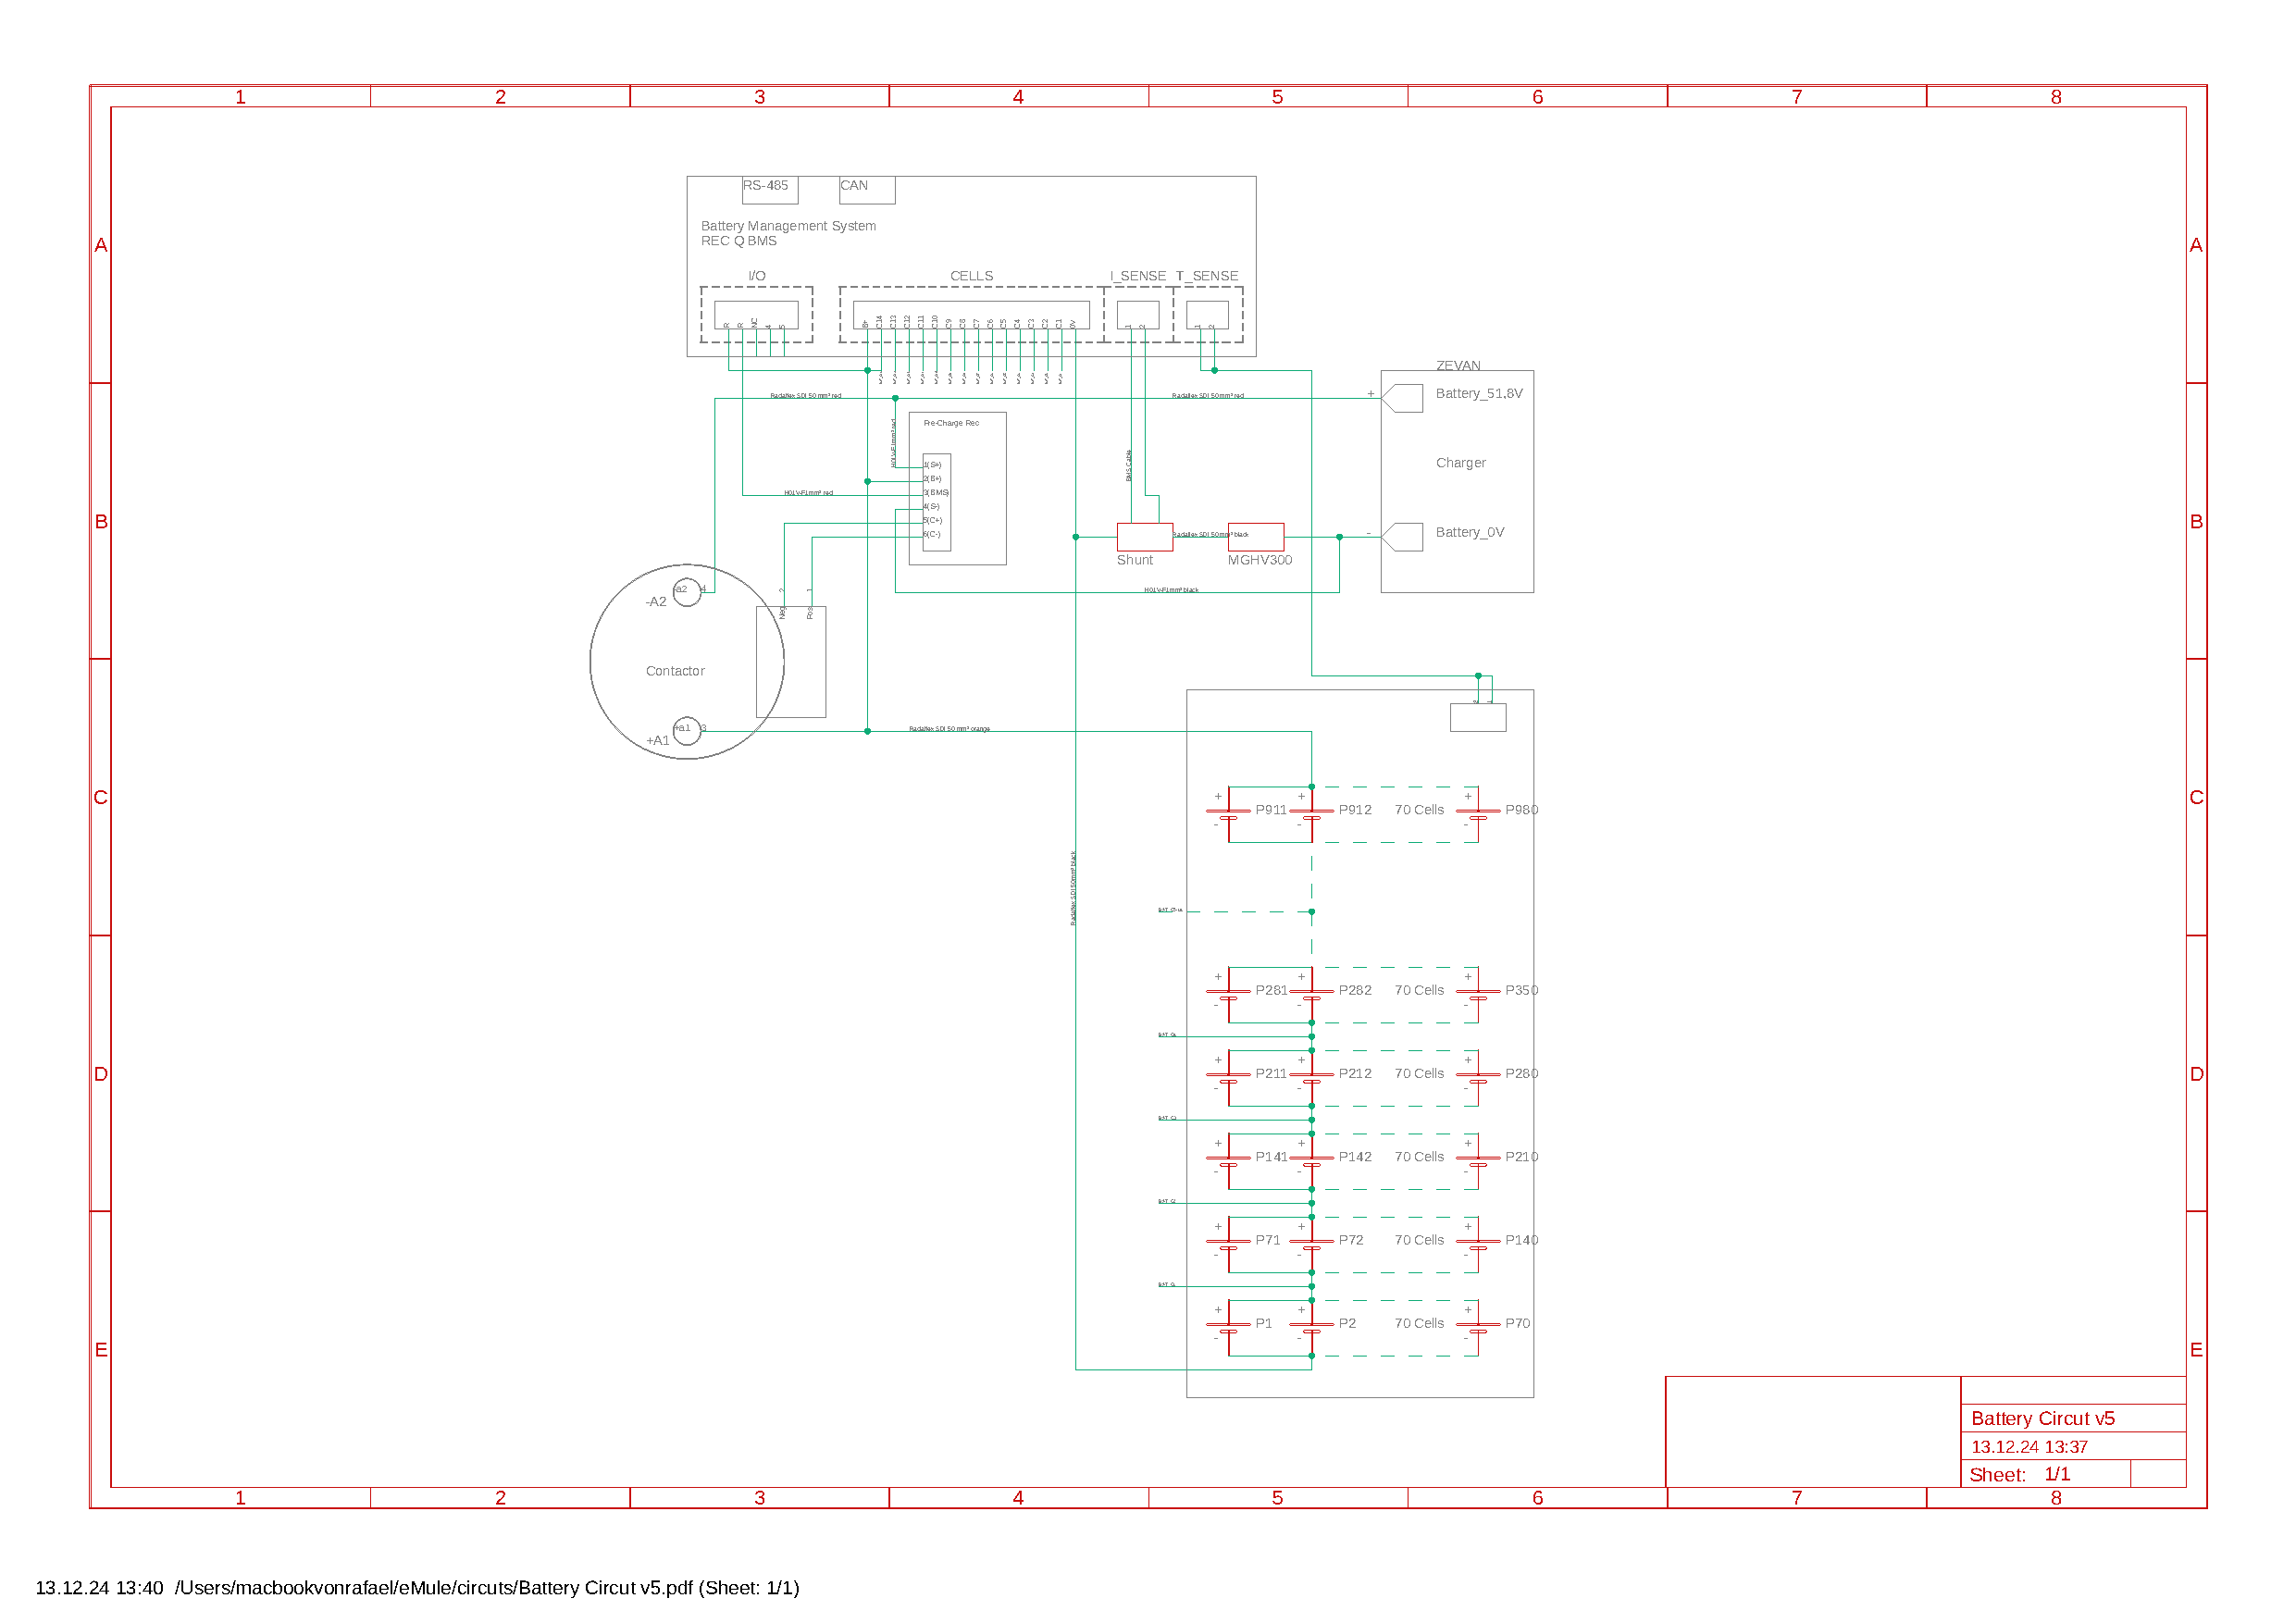
\includepdf[pages=1, trim=0cm 0cm 21cm 0cm, clip]{circuts/Battery Circut v5.pdf}

% Rechte Hälfte der A3-Seite
%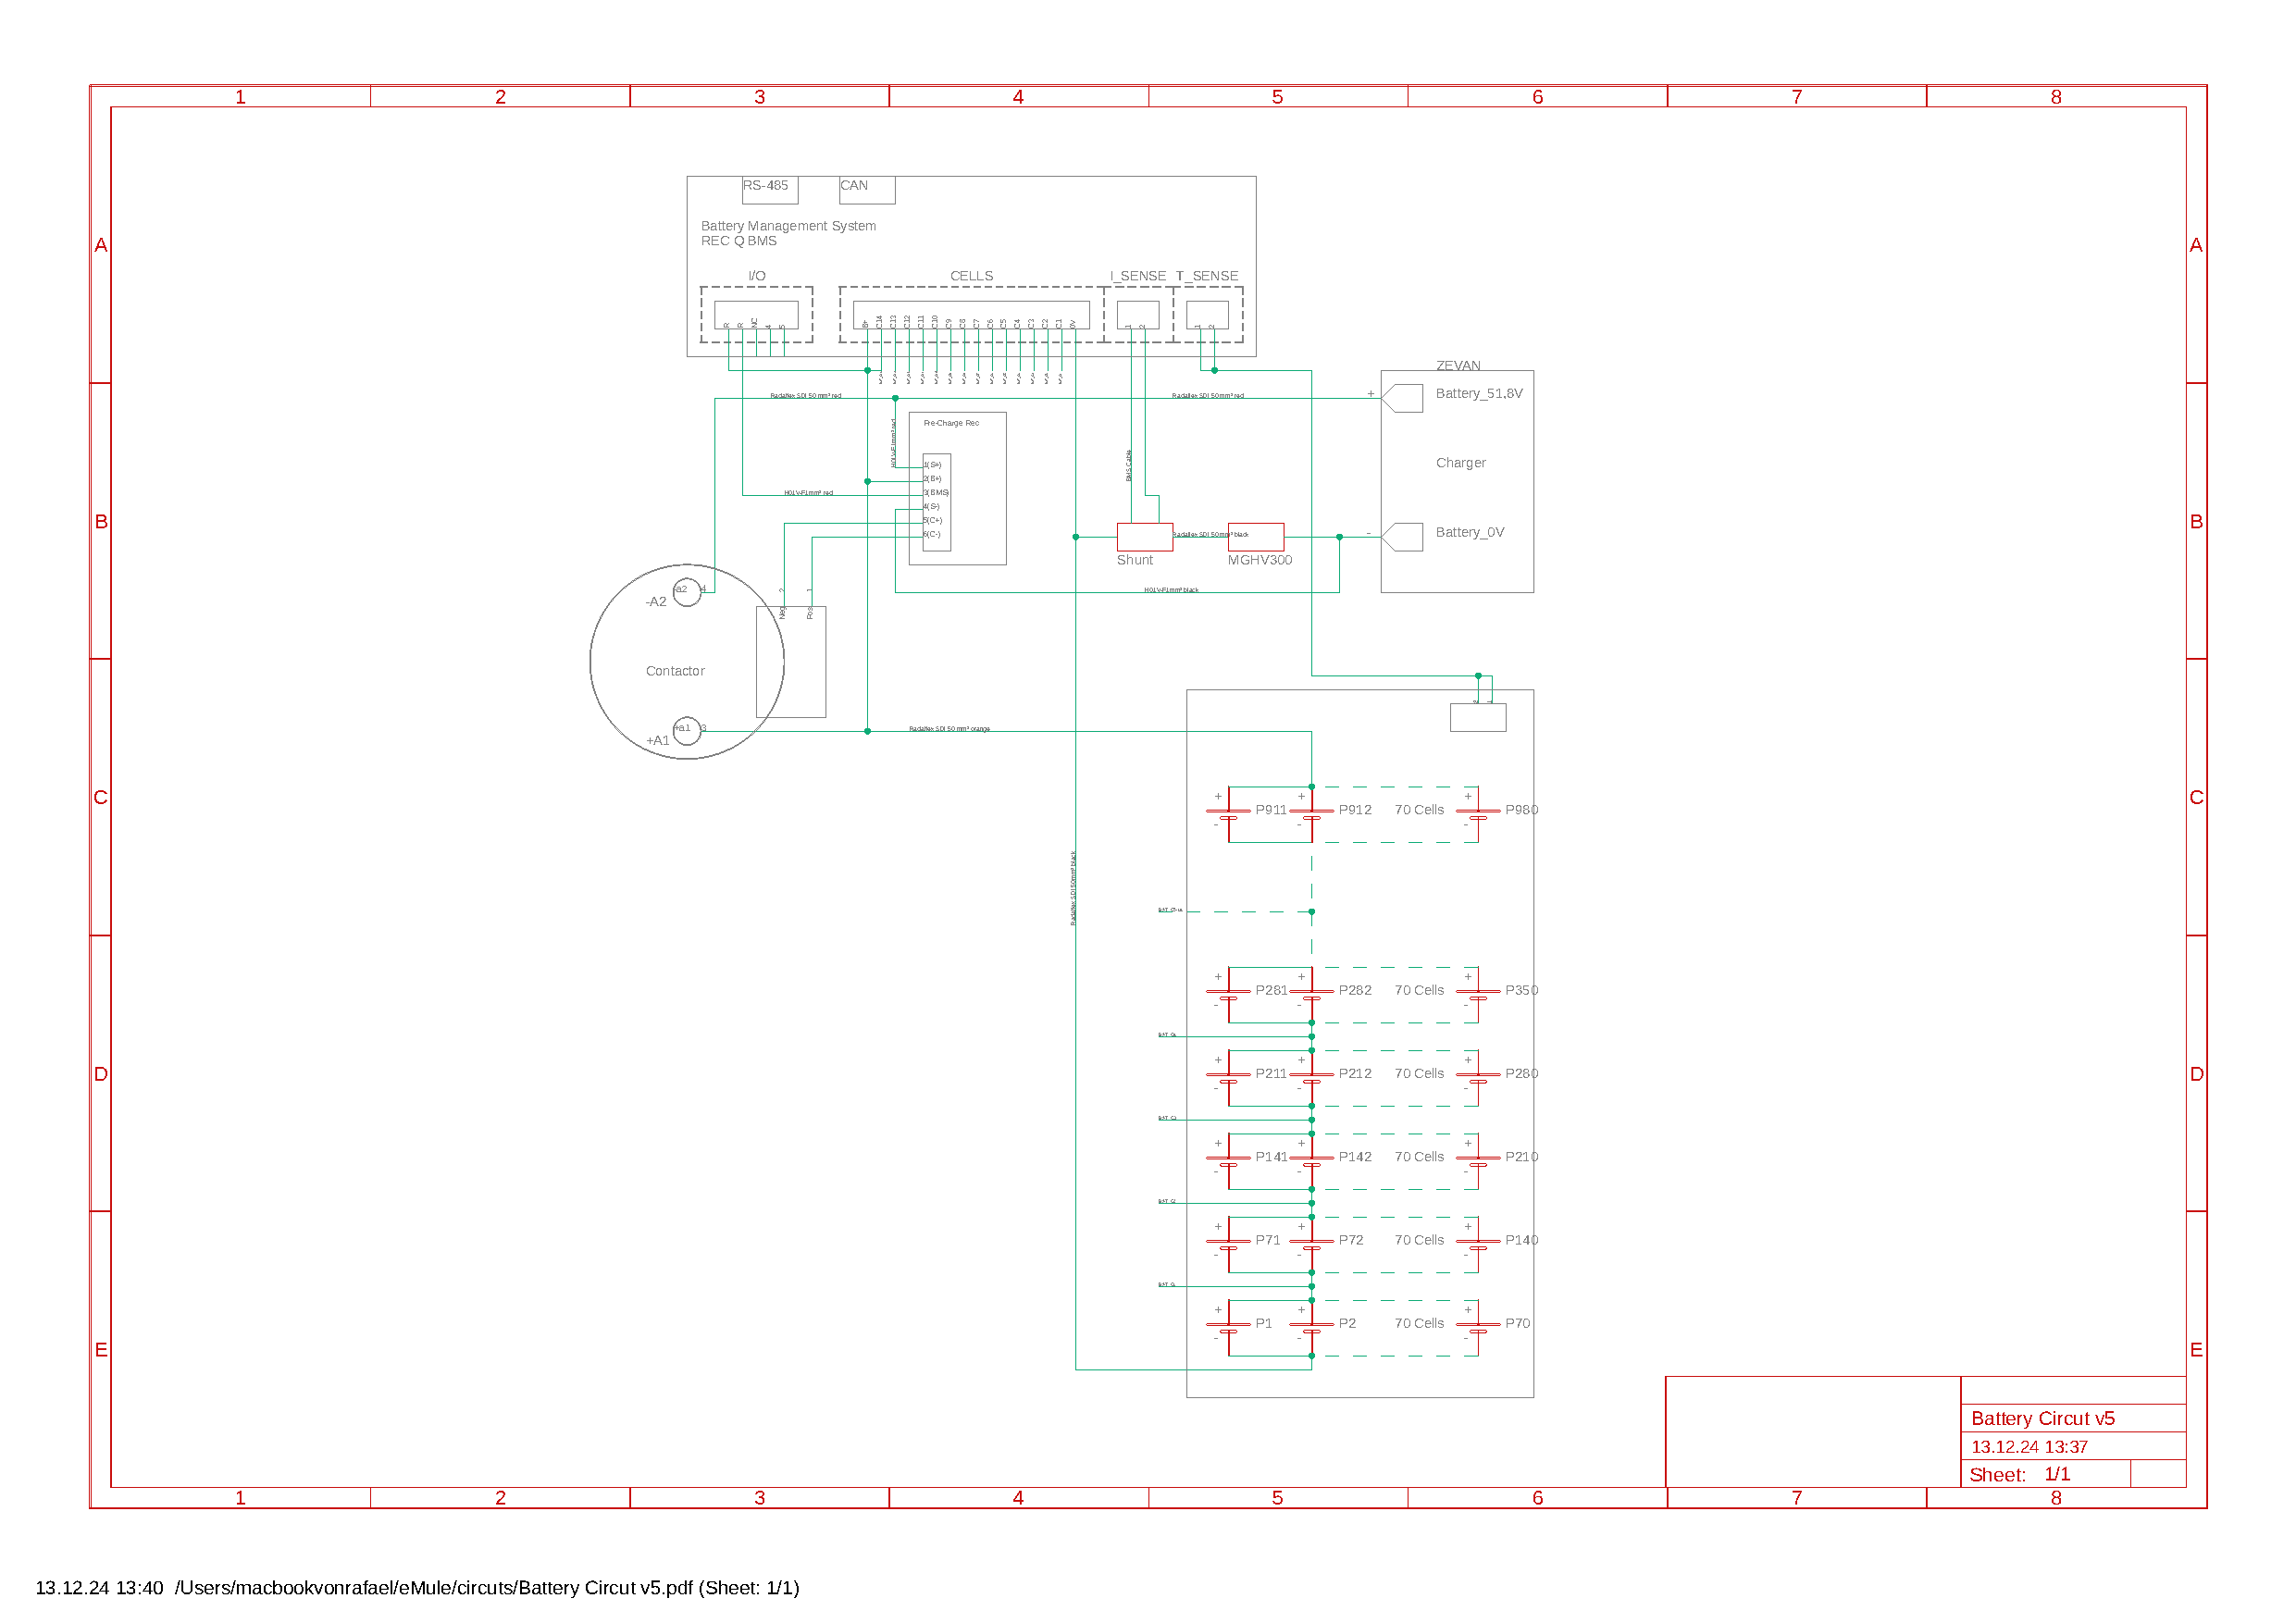
\includepdf[pages=1, trim=21cm 0cm 0cm 0cm, clip]{circuts/Battery Circut v5.pdf}

%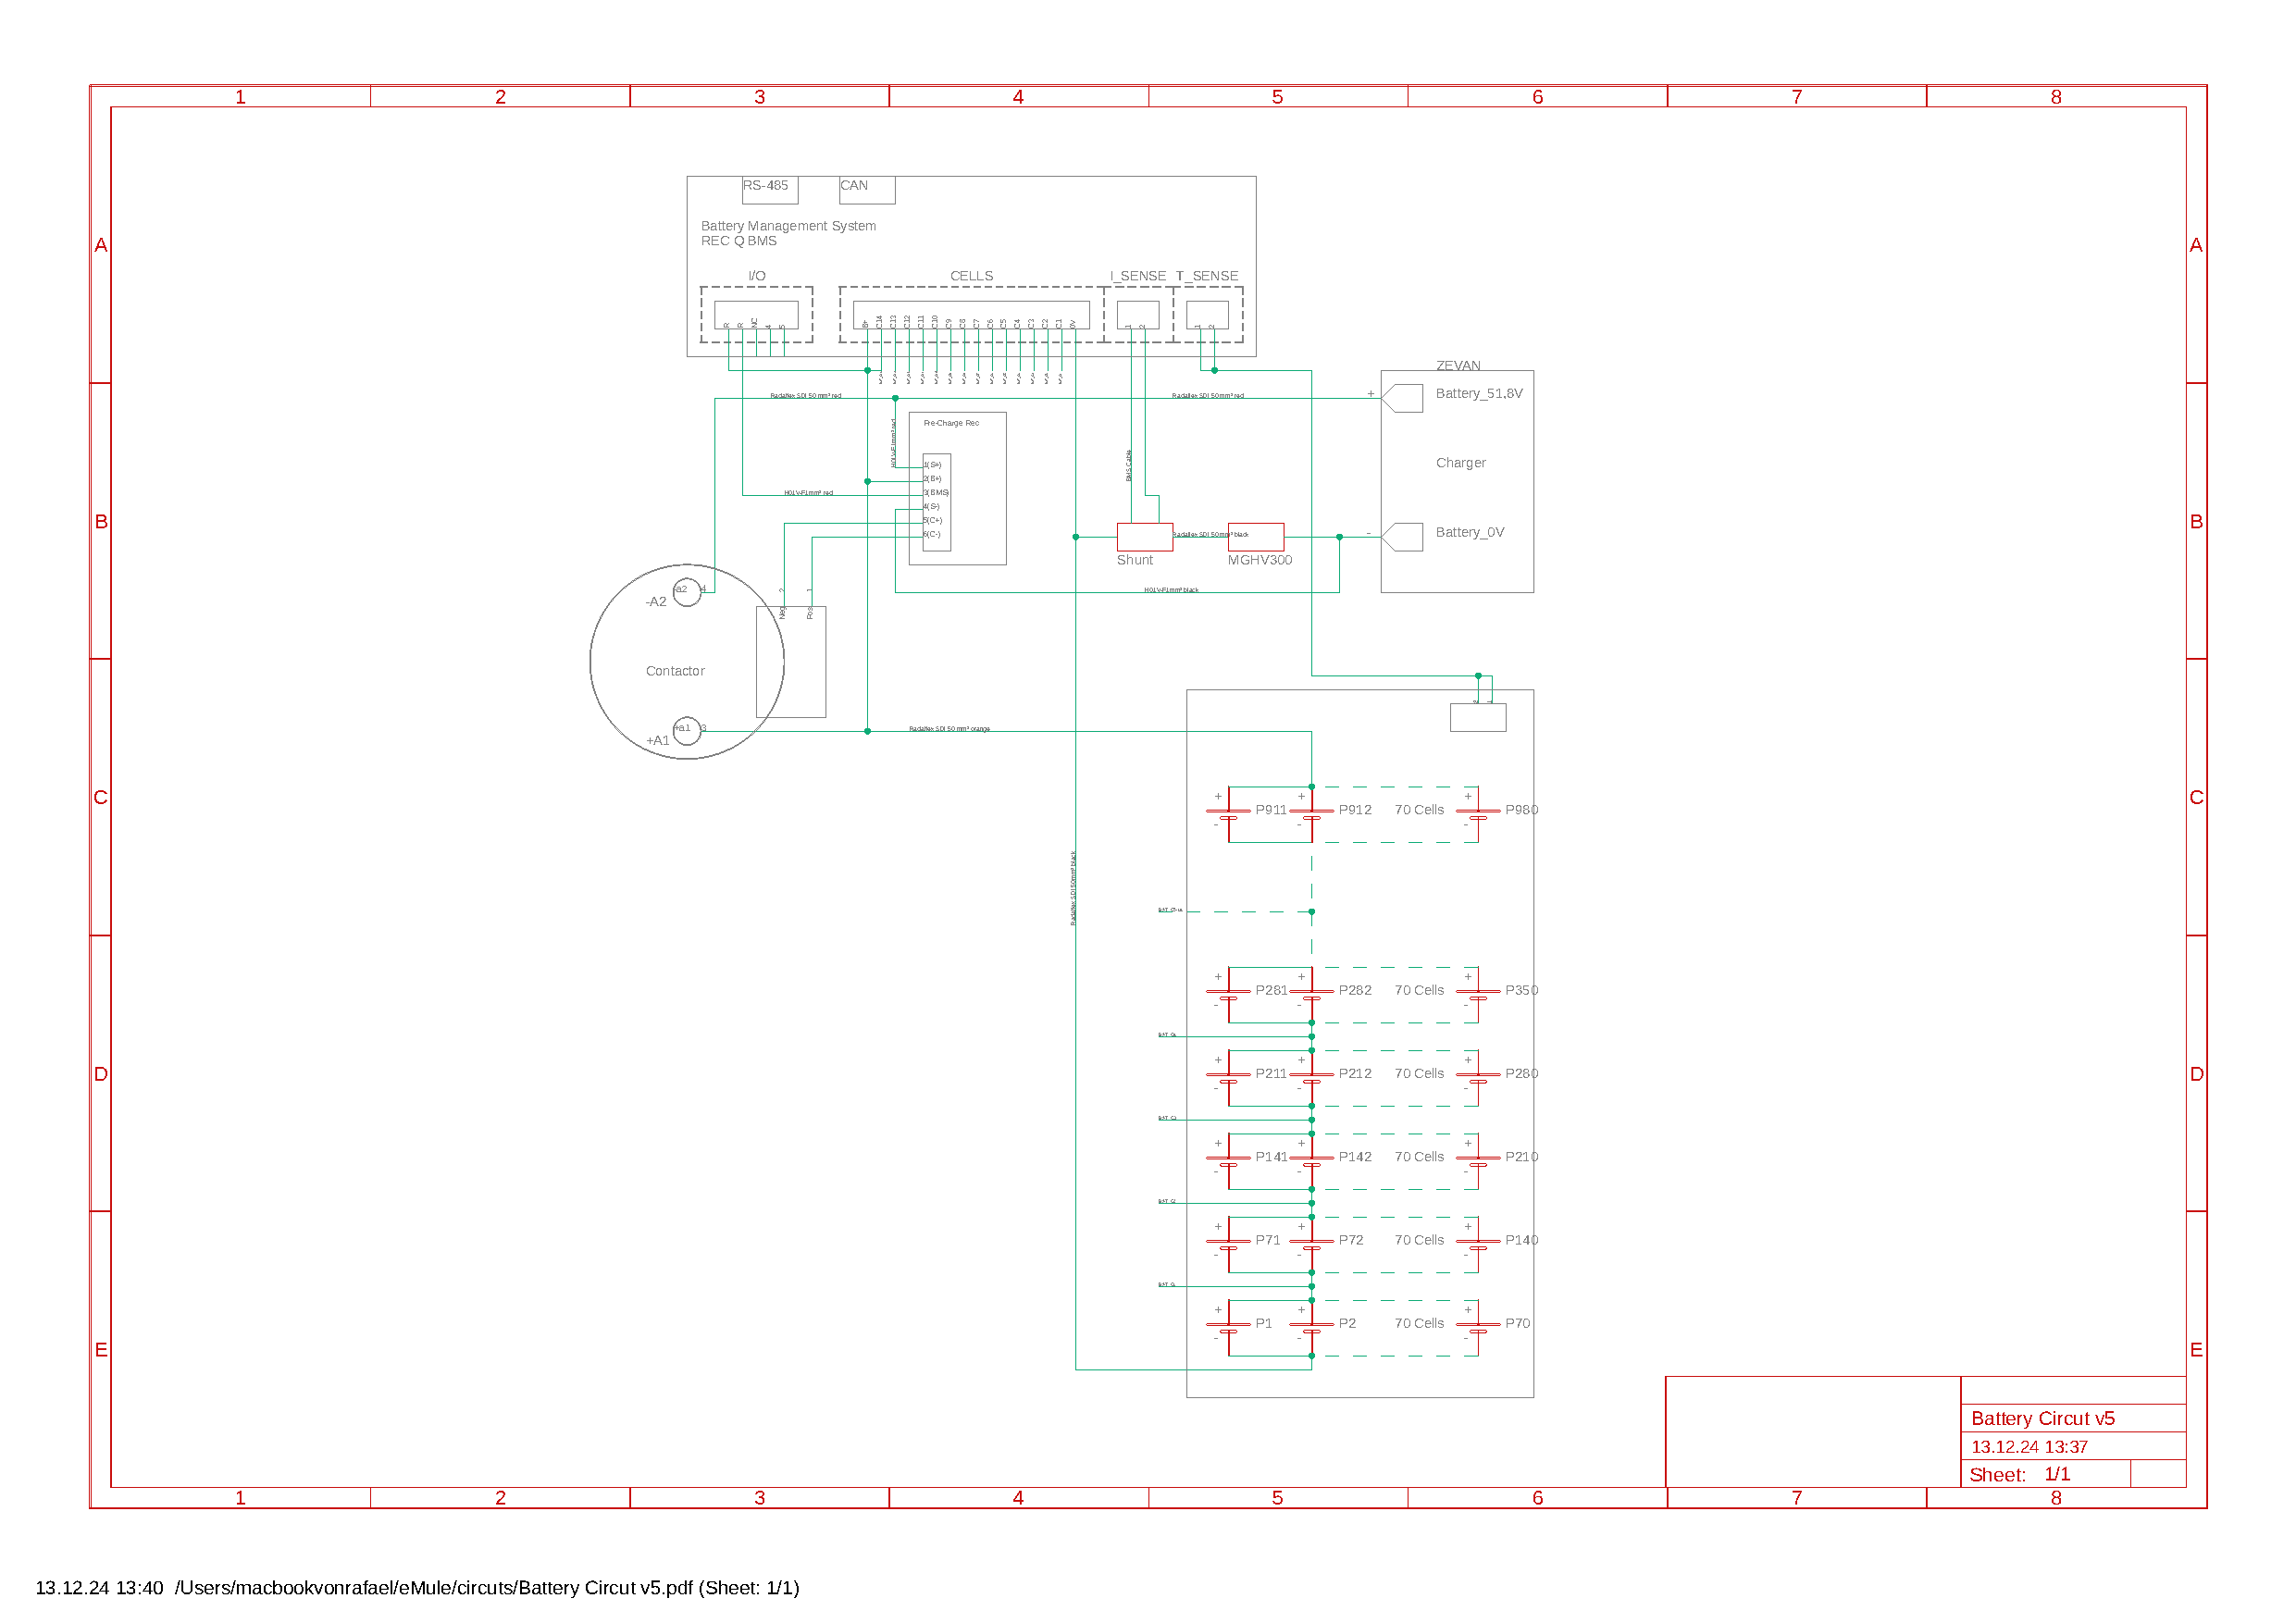
\includepdf[pages=1, angle=90, fitpaper=true]{circuts/Battery Circut v5.pdf}

\section*{Schaltplan Batterie Circuit}
Für die umsetzung des Battery Circut Stromlauftplans muss im ersten Schritt der vorhandene Schaltplan auf Fehler überprüft werden. Um dies möglichst effizient zu gestalten wird der Stromlaufplan ausgedruckt.Gefundene Fehler werden im nächsten Schritt markiert und korrigiert. Sind alle Fehler korrigiert, muss der Stromlaufplan so angepasst werden, dass die bestmögliche Übersichtlichkeit entsteht. Im letzten Schritt muss herausgefunden werden, nach welcher Norm der Stromlaufplan erstellt wurde. Diese Norm muss recherchiert und in die von uns gewählte DIN EN 60617 Norm \glqq übersetzt\grqq {} werden. Sind sämtliche Schritte absolviert kann der Schaltplan mit Hilfe von Autodesk Fusion 360 in den gewünschten Rahmen, hier DIN A3, eingefügt werden.
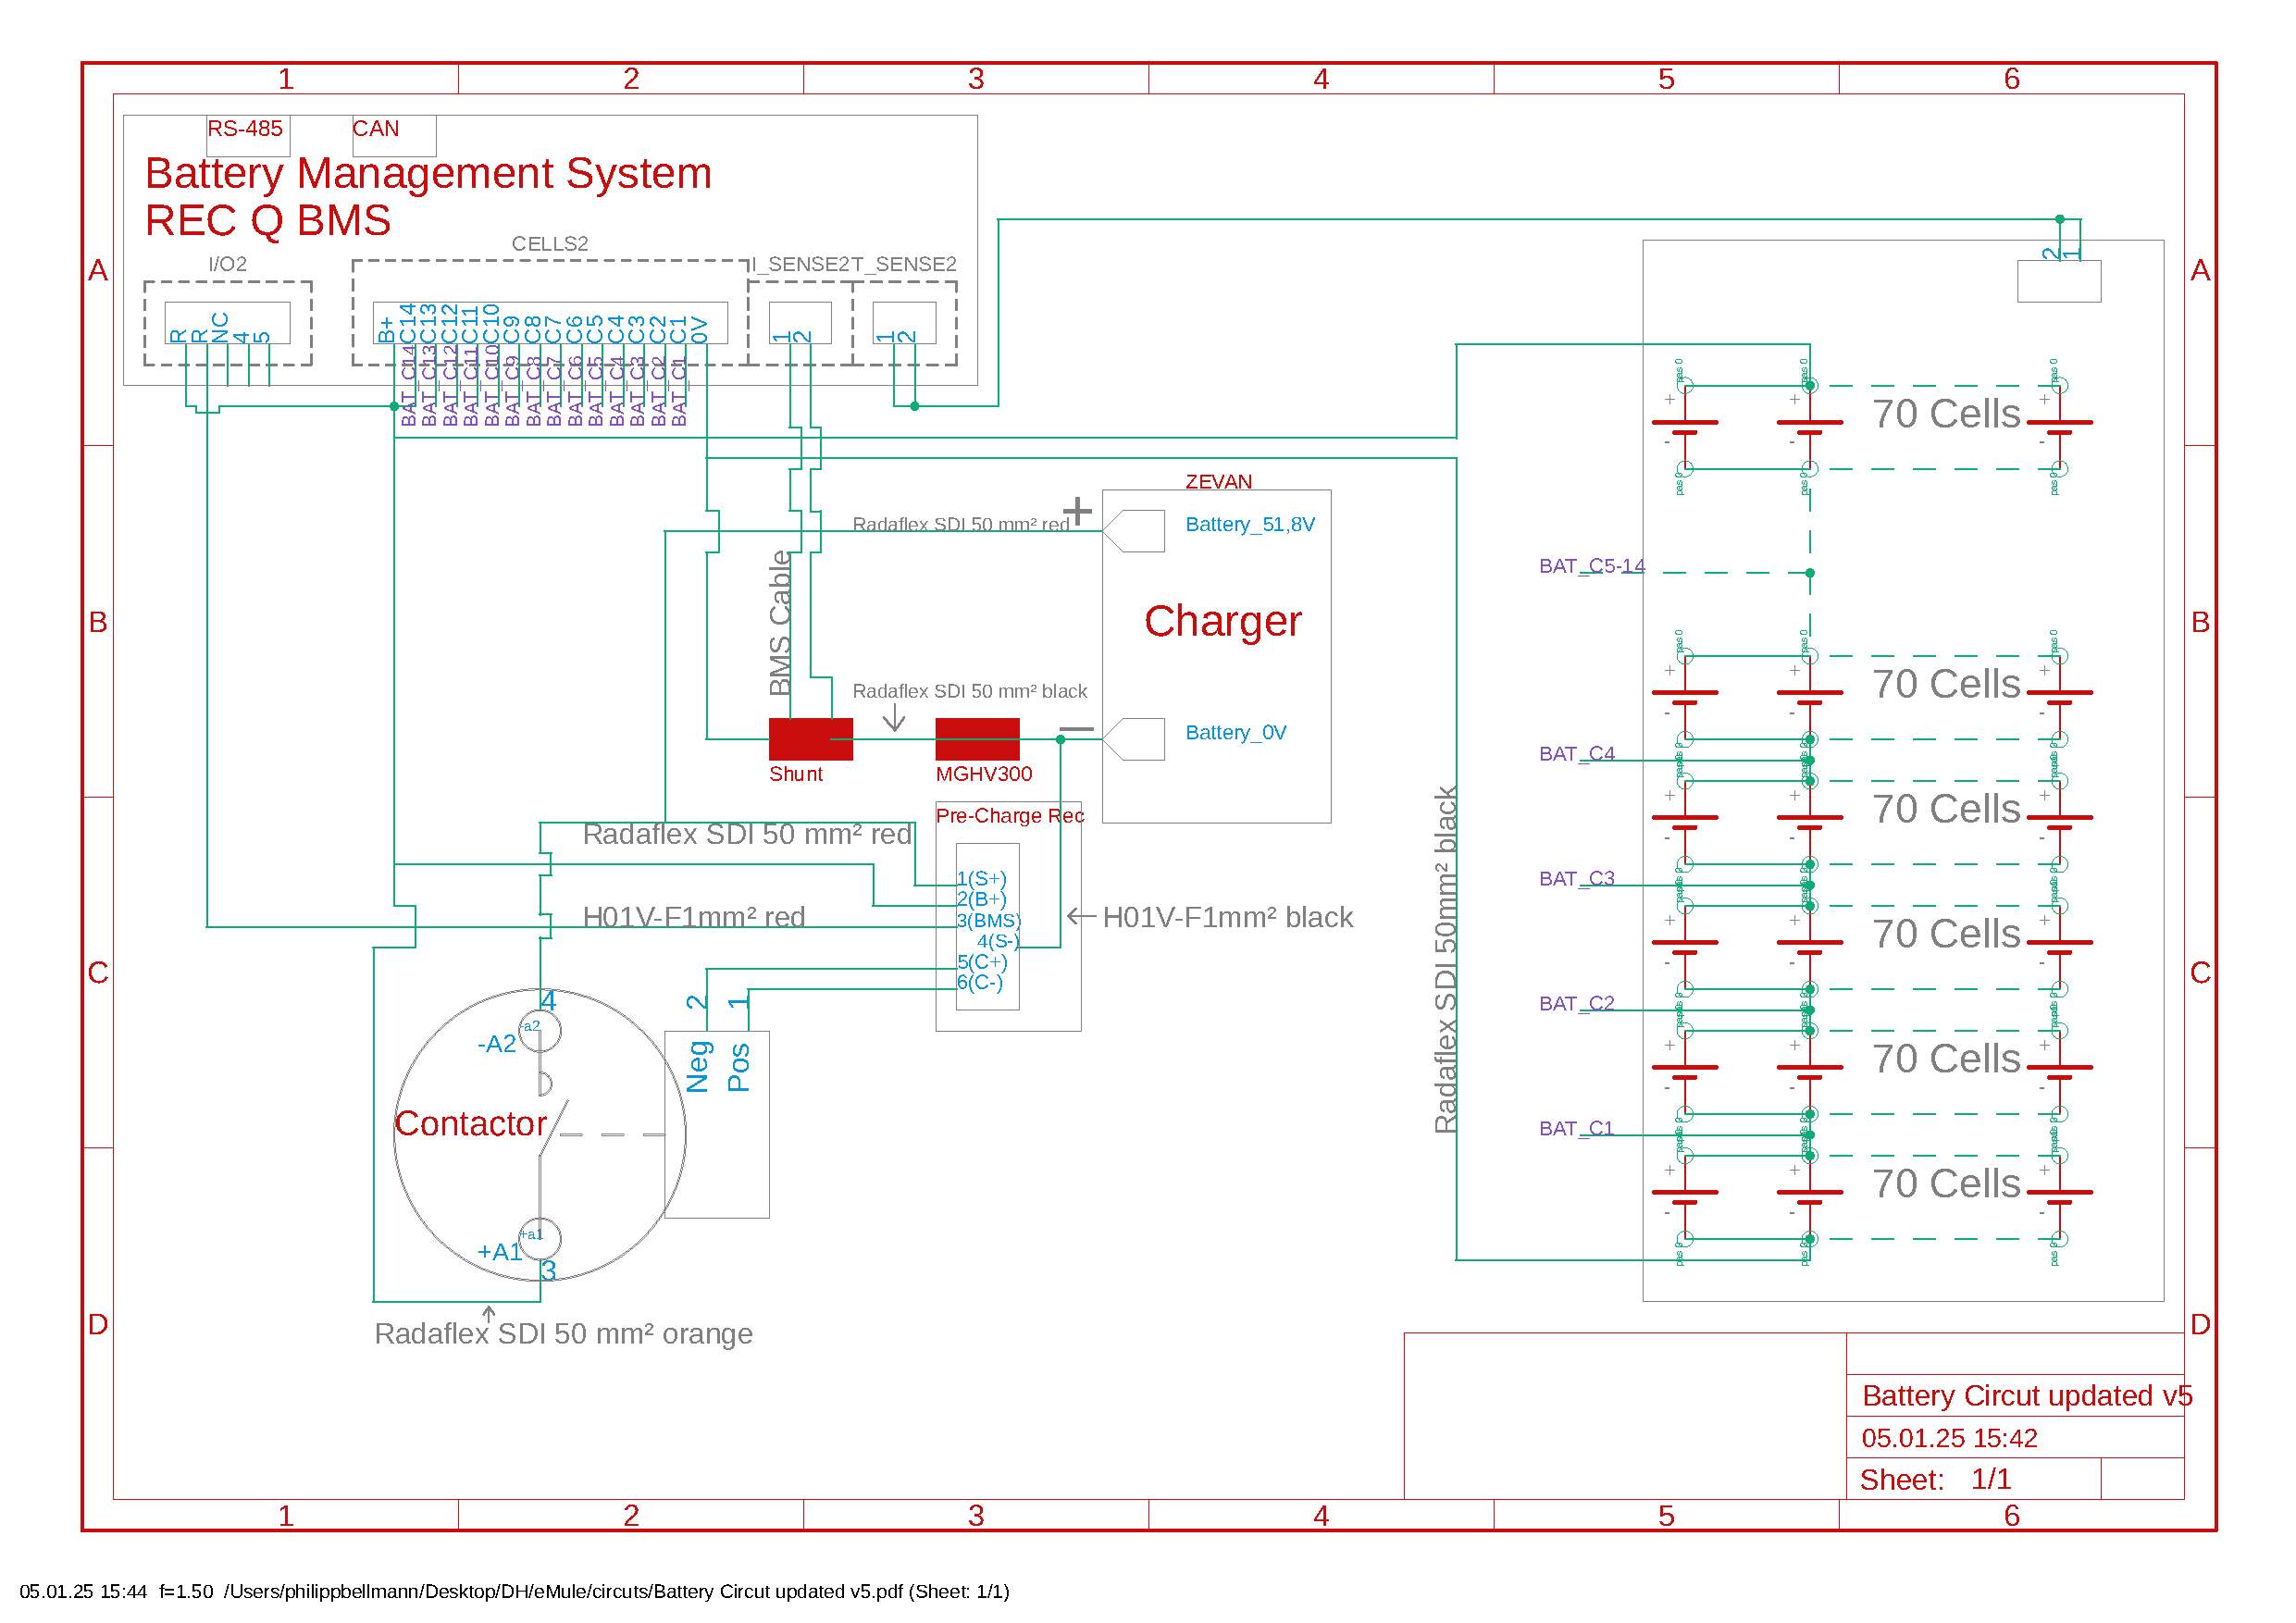
\includepdf[pages=1, fitpaper=true]{circuts/Battery Circut updated.pdf} 

\addtocounter{page}{1} 
\section*{Schaltplan Motor Controller}
Zur Analyse und Bearbeitung des Stromlaufplans „Motor Controller“ wird der Plan zunächst ausgedruckt und systematisch auf Unstimmigkeiten, wie fehlende Verbindungen oder unklare Symbolik, überprüft. Gefundene Fehler werden markiert und anschließend korrigiert, wobei die Einhaltung elektrotechnischer Standards gewährleistet wird. Zudem erfolgt eine Layoutanpassung zur Verbesserung der Übersichtlichkeit. Im nächsten Schritt wird geprüft, ob der Schaltplan den Vorgaben der DIN EN 60617 entspricht. Abweichungen werden identifiziert und normgerecht angepasst. Der überarbeitete Schaltplan wird schließlich mit Autodesk Fusion 360 in ein DIN-A3-Format übertragen. Dabei werden Titelblock und Legende integriert, um die Professionalität und Lesbarkeit sicherzustellen. 
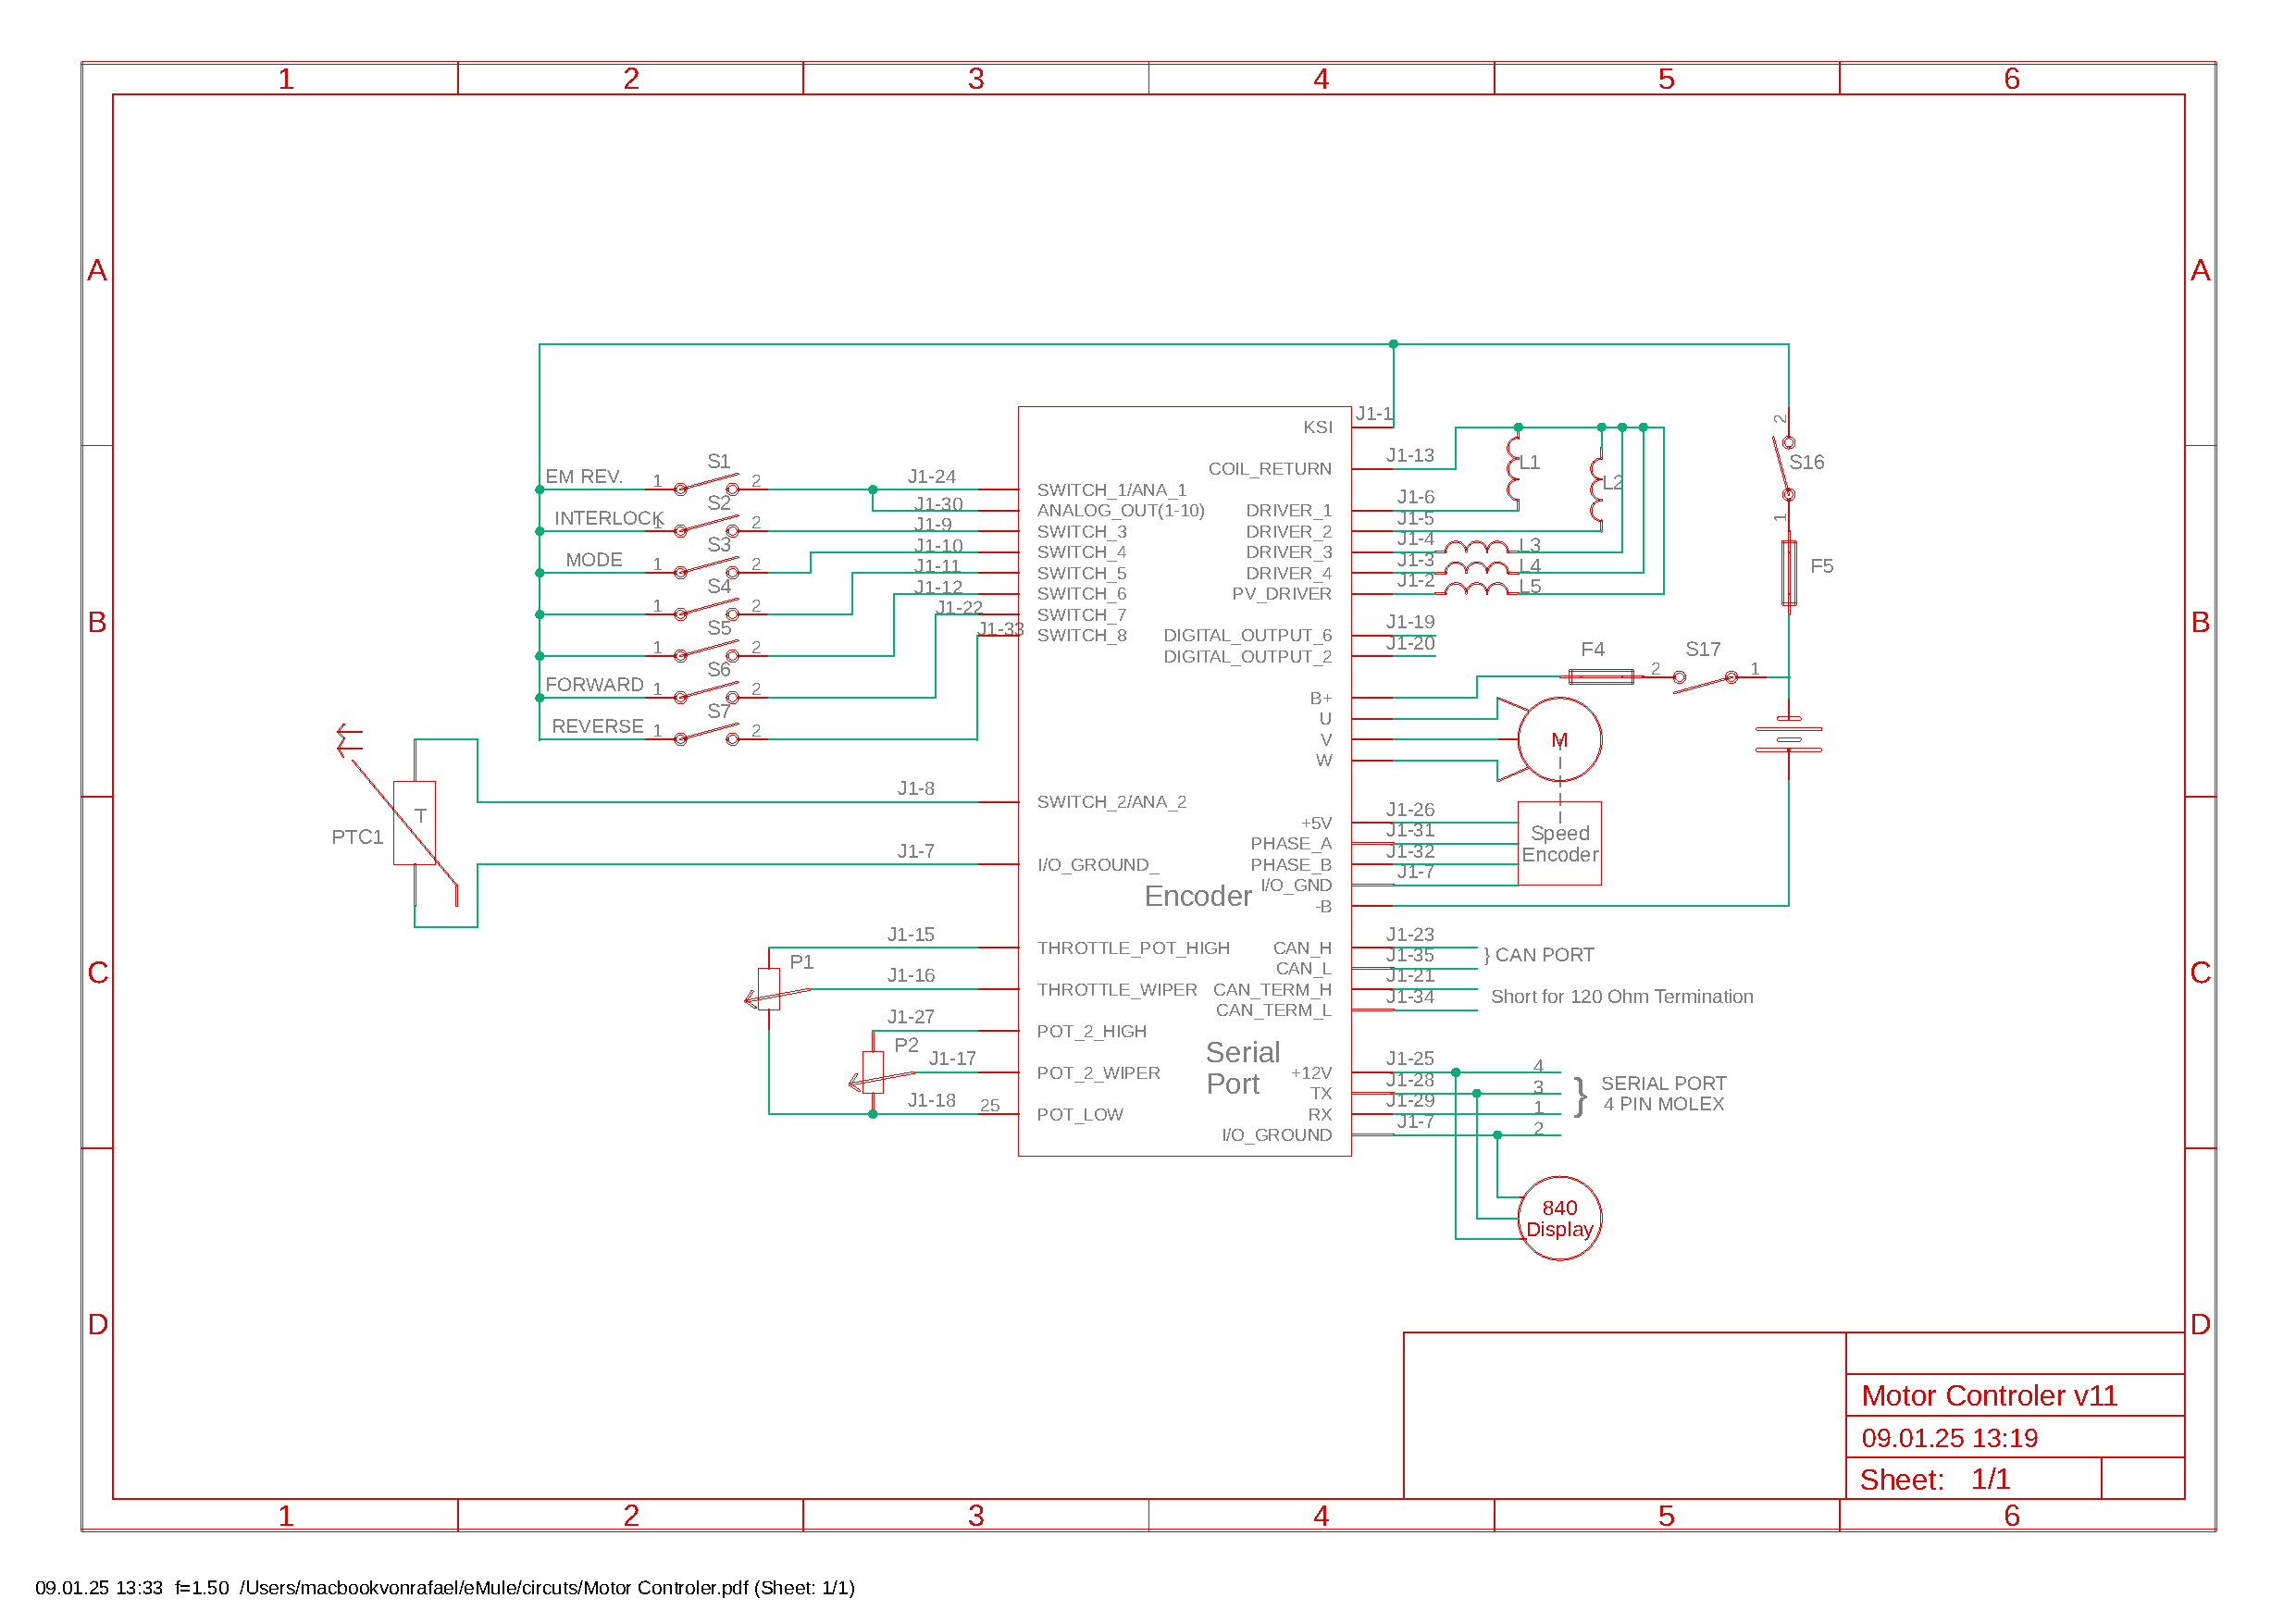
\includepdf[pages=1, fitpaper=true]{circuts/Motor Controler.pdf} 
\addtocounter{page}{1} 
\section*{Schaltplan Onboard-Netz}
Der Stromlaufplan „Onboard-Netz“ wird nach dem gleichen Vorgehen wie bei den vorherigen Plänen bearbeitet, wobei der Schwerpunkt auf der Lesbarkeit liegt. Nach der Fehlerprüfung und -korrektur wird das Layout so überarbeitet, dass Verbindungen und Beschriftungen klarer und übersichtlicher dargestellt werden. Normgerechte Anpassungen nach DIN EN 60617 und die Übertragung in ein DIN-A3-Format stellen sicher, dass der Schaltplan nicht nur funktional, sondern auch optimal lesbar ist.
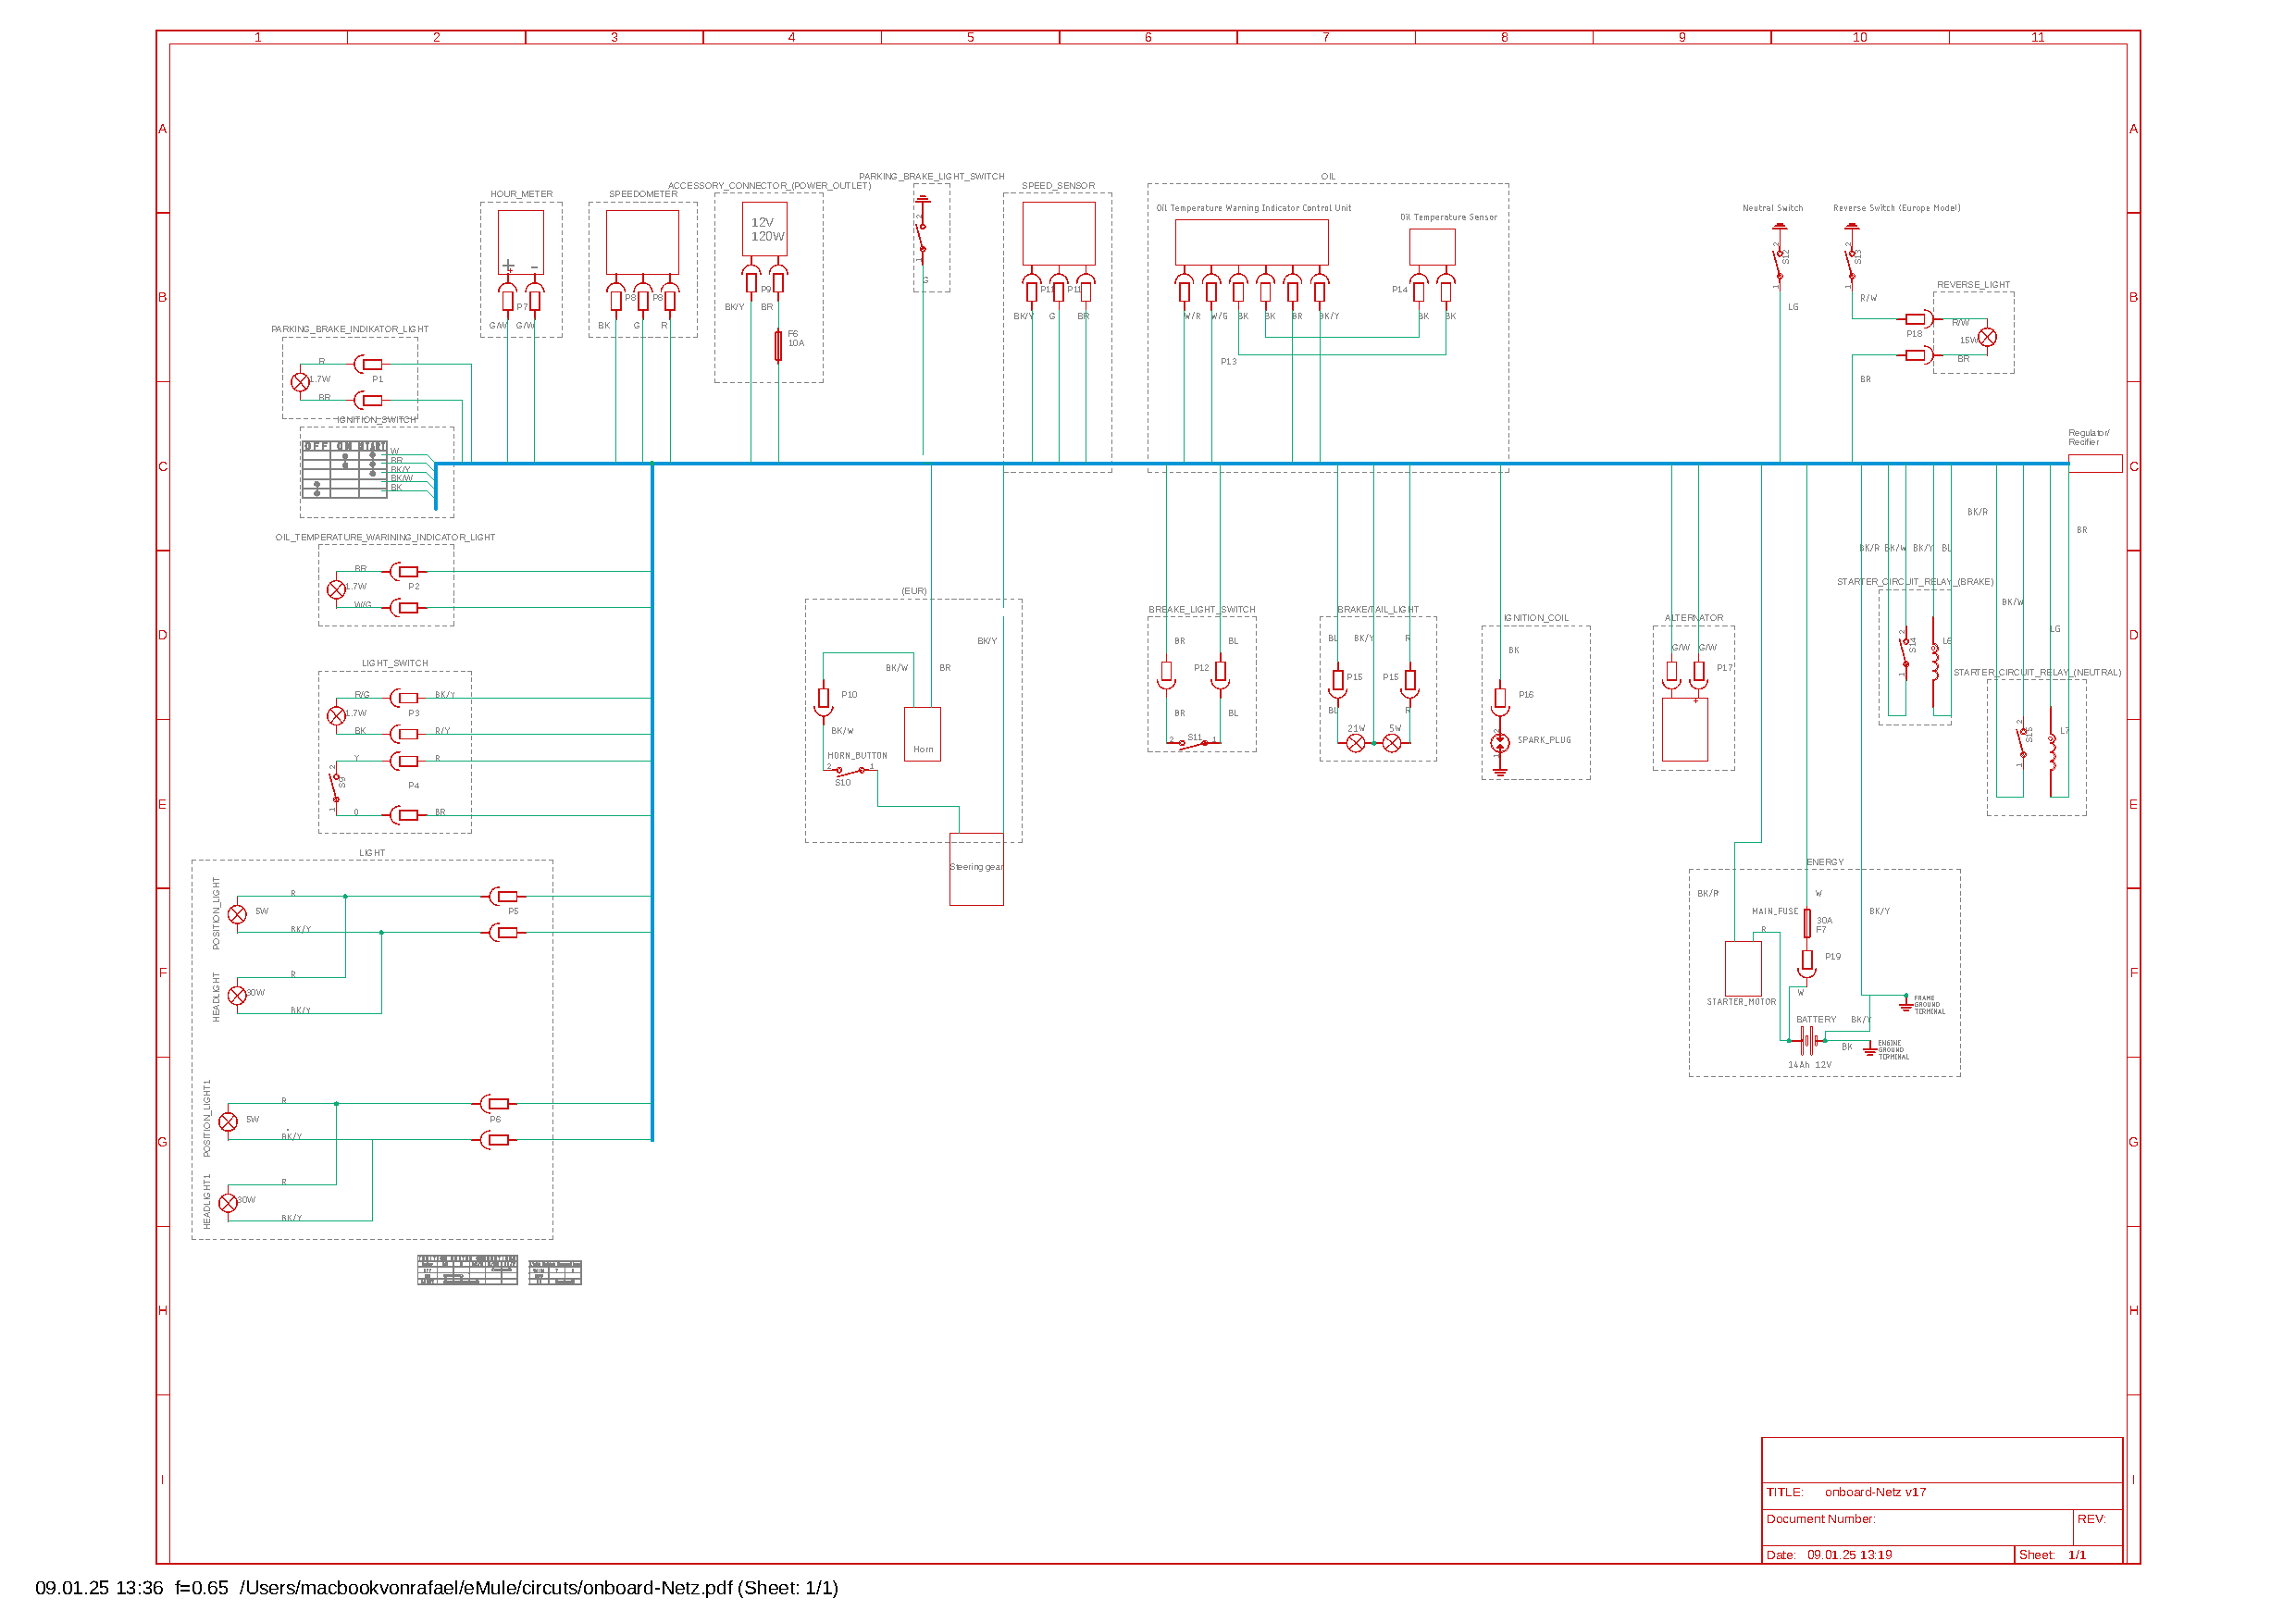
\includepdf[pages=1, fitpaper=true]{circuts/onboard-Netz.pdf} 
\addtocounter{page}{1} 
\section*{Temperatursteuerung des Ladegeräts}
Der Schaltplan zur Temperatursteuerung des Ladegeräts wird gemäß der Norm DIN EN 60617 erstellt. Diese Norm definiert die symmetrische Darstellung von Schaltungen und sorgt für eine klare, standardisierte Kommunikation im Bereich der Elektrotechnik. Der Schaltplan beinhaltet einen Temperatursensor, der die Temperatur des Ladegeräts misst. Bei Überschreitung eines festgelegten Temperaturwerts wird ein Steuermechanismus aktiviert, der entweder die Kühlung einleitet oder das Ladegerät abschaltet, um eine Überhitzung zu verhindern und die Sicherheit sowie die Lebensdauer der Geräte zu gewährleisten.
%\includepdf[pages=1, fitpaper=true]{circuts/Temperatursteuerung des Ladegerätes.pdf} 
\addtocounter{page}{1} 
\section*{HV-Onboard-Netz}

Der Schaltplan für ein Ladegerät mit HV-Onboard-Netz wird gemäß der Norm DIN EN 60617 erstellt. In diesem Schaltplan werden alle relevanten elektrischen Komponenten, die für den Betrieb eines Hochvolt-Onboard-Netzes erforderlich sind, standardisiert dargestellt. Dazu gehören die Spannungsversorgungseinheit, die Schutzschaltungen, die Kommunikationsschnittstellen sowie die Schnittstellen für die Steuerung und Überwachung des Hochvoltnetzes. Die Norm sorgt dafür, dass die Schaltung klar verständlich und international kompatibel ist, um die Sicherheit und Effizienz des gesamten Systems zu gewährleisten.
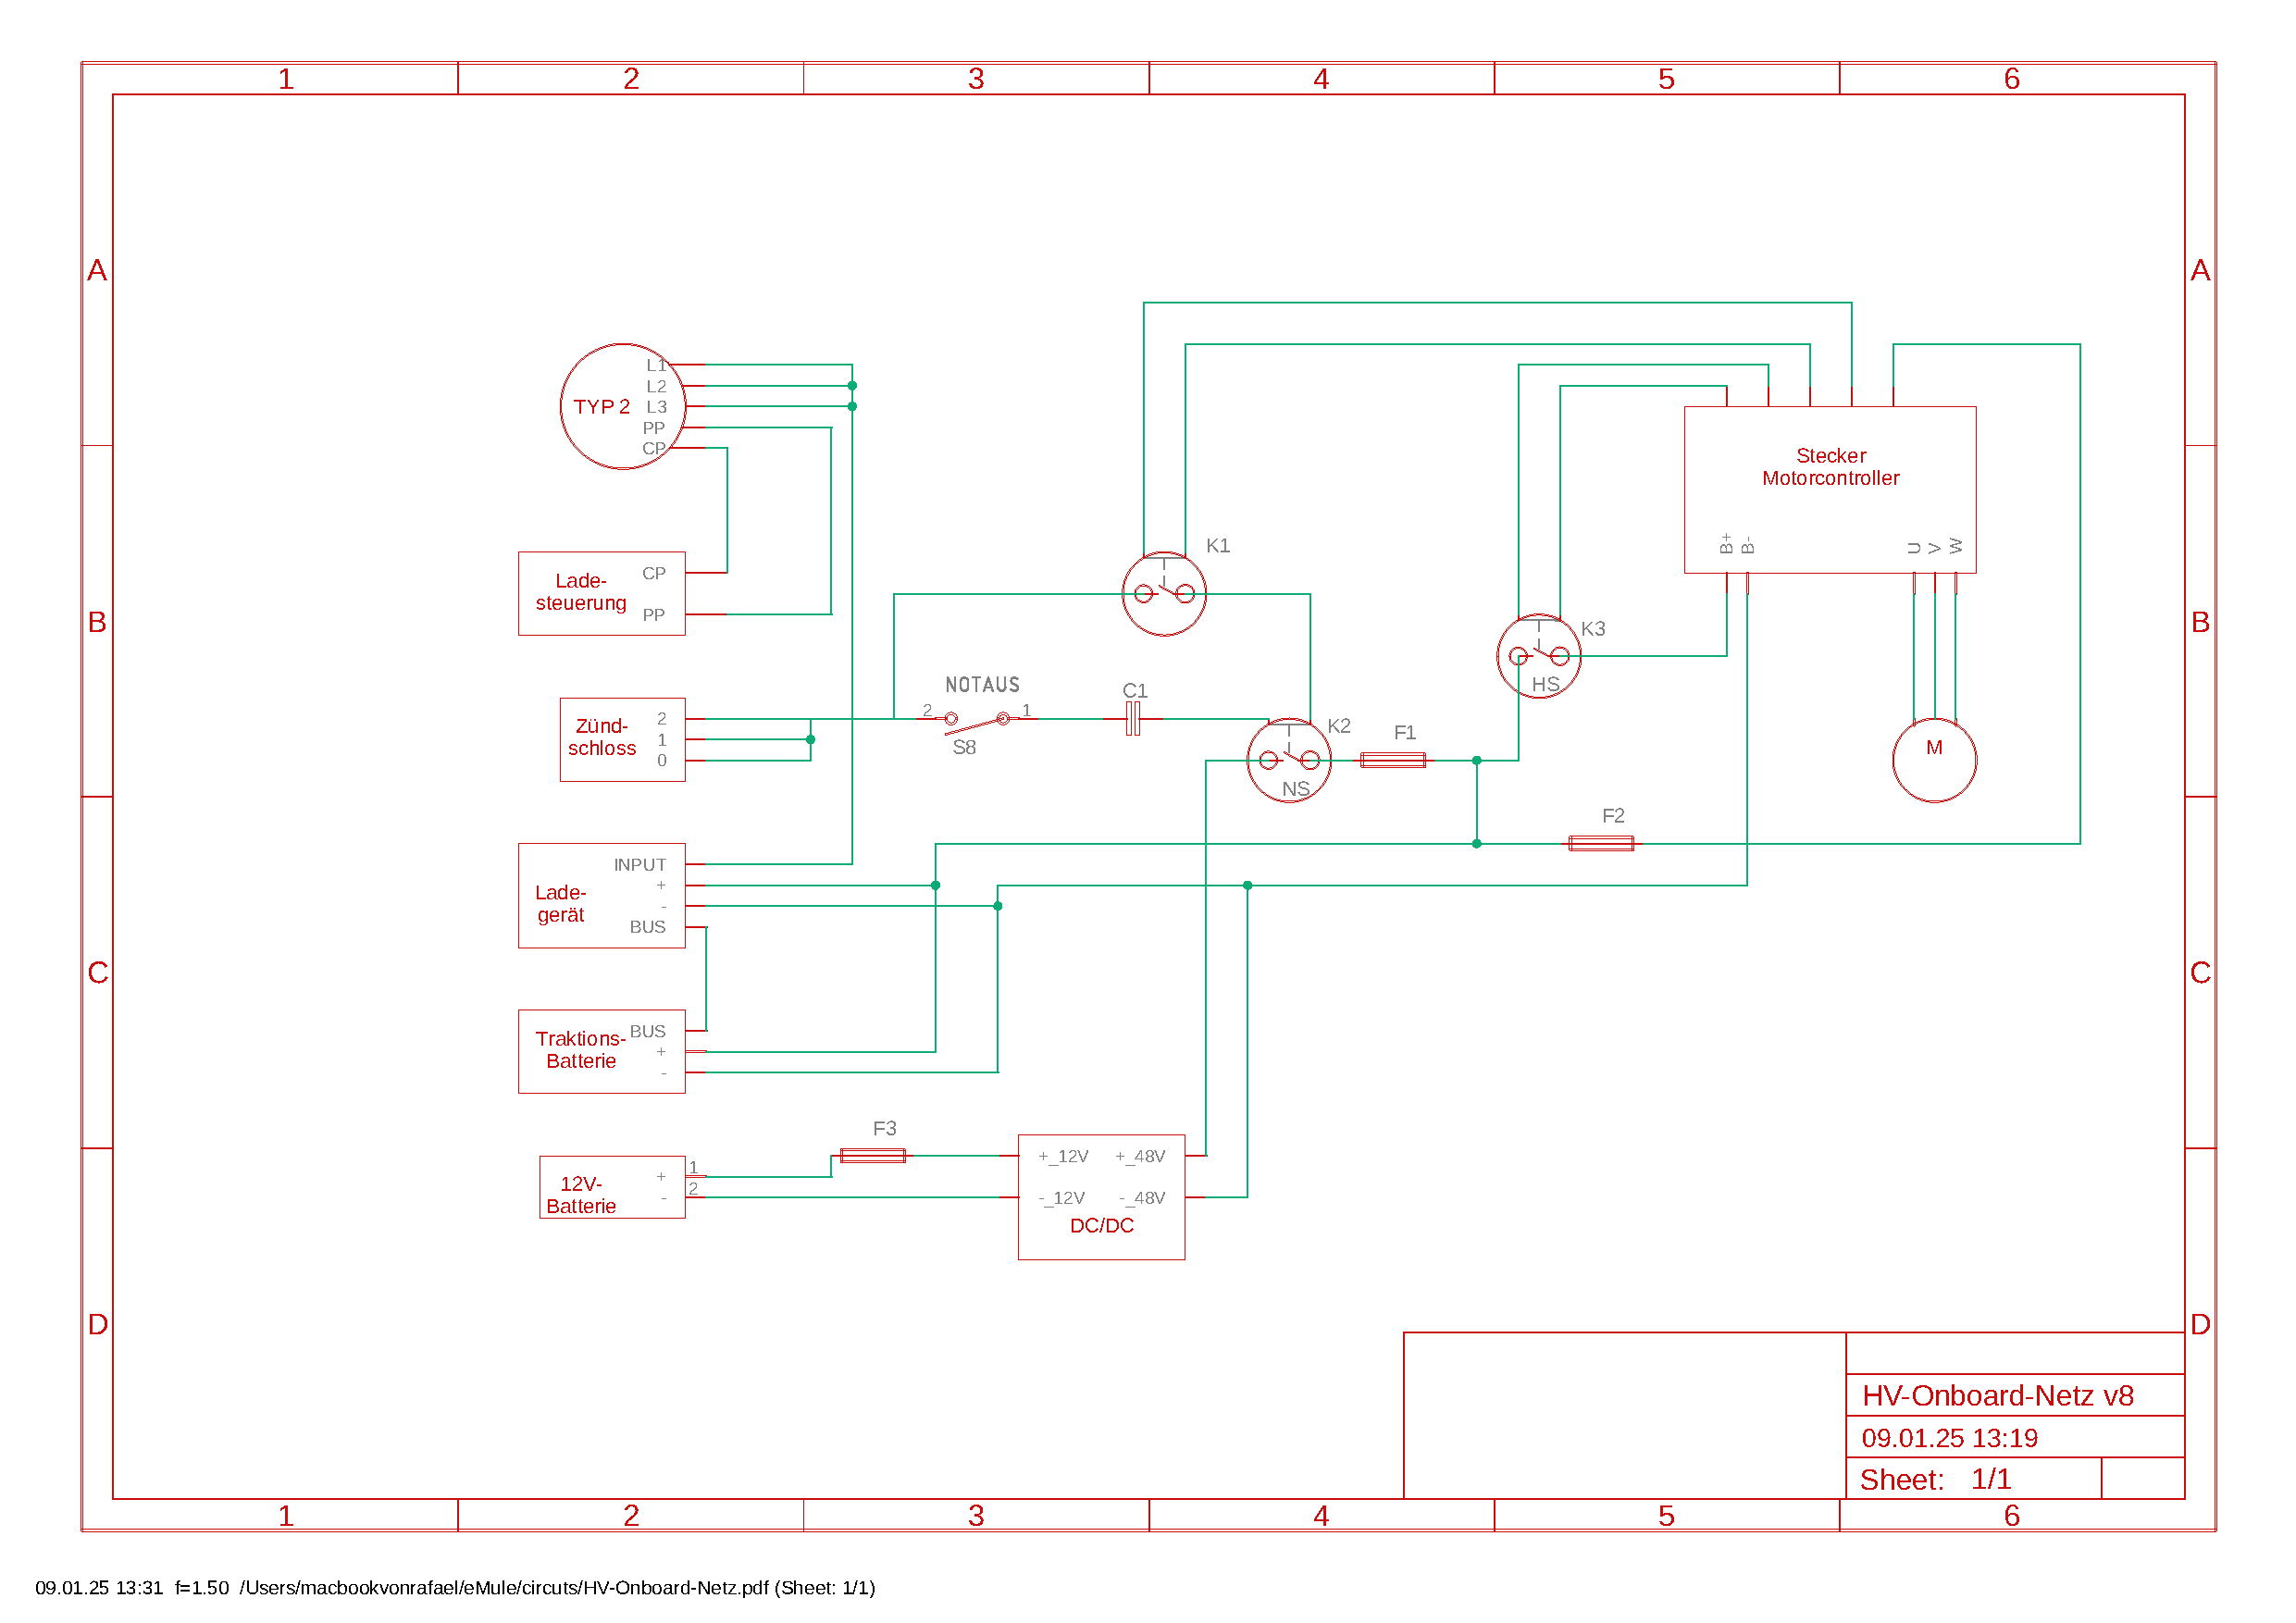
\includepdf[pages=1, fitpaper=true]{circuts/HV-Onboard-Netz.pdf} 
\addtocounter{page}{1} 
\section*{Legende der Schaltzeichen}
In der folgenden Tabelle werden die verwendeten Schaltzeichen des Schaltplans gemäß der Norm DIN EN 60617 erläutert. Diese Schaltzeichen dienen dazu, die elektrischen Komponenten und deren Verbindungen im Schaltplan eindeutig und standardisiert darzustellen. Die Legende bietet eine Übersicht über die Symbole, die in den darauffolgenden Schaltplänen verwendet werden, und erleichtert so das Verständnis der Systemarchitektur und Funktionalität des Hochvolt-Onboard-Netzes.
\begin{table}[ht]
	\centering
	\resizebox{0.75\textwidth}{!}{% Verkleinert die gesamte Tabelle auf 90 % der Textbreite
		\renewcommand{\arraystretch}{1.8}
		\setlength{\tabcolsep}{15pt}
		\begin{tabular}{|m{5cm}|m{7cm}|}
			\hline
			\textbf{Symbol} & \textbf{Beschreibung} \\
			\hline
			\centering\includegraphics[width=2cm]{Legende/Schütz.png} & \centering Schütz \tabularnewline
			\hline
			\centering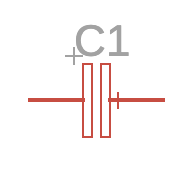
\includegraphics[width=2cm]{Legende/Kondensator.png} & \centering Kondensator \tabularnewline
			\hline
			\centering
\includegraphics[width=2cm]{Legende/Funkenstrecke.png} & \centering Funkenstrecke \tabularnewline
			\hline
			\centering
\includegraphics[width=2cm]{Legende/Ground.png} & \centering Masse (Ground) \tabularnewline
			\hline
			\centering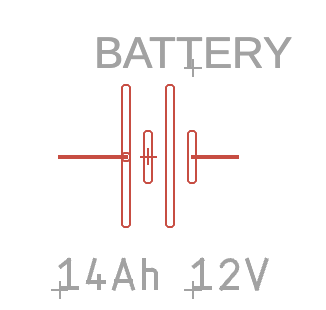
\includegraphics[width=2cm]{Legende/Batterie.png} & \centering Batterie \tabularnewline
			\hline
			\centering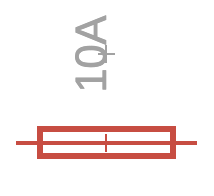
\includegraphics[width=2cm]{Legende/Sicherung.png} & \centering Sicherung \tabularnewline
			\hline
			\centering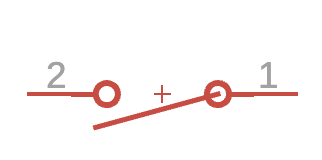
\includegraphics[width=2cm]{Legende/Schalter.png} & \centering Schalter \tabularnewline
			\hline
			\centering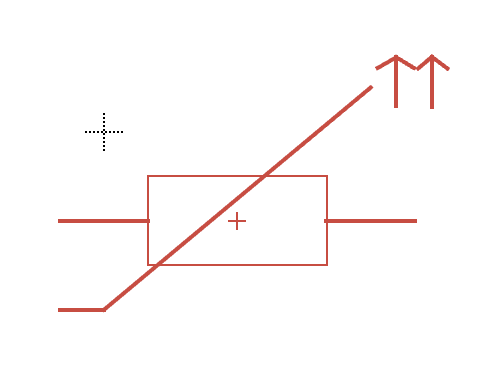
\includegraphics[width=2cm]{Legende/PTC-Widerstand.png} & \centering PTC-Widerstand \tabularnewline
			\hline
			\centering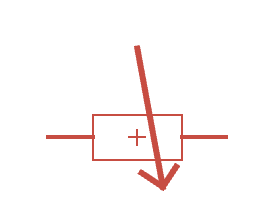
\includegraphics[width=2cm]{Legende/Potentiometer.png} & \centering Potentiometer \tabularnewline
			\hline
			\centering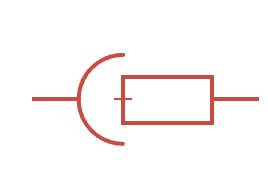
\includegraphics[width=2cm]{Legende/Stecker.png} & \centering Stecker \tabularnewline
			\hline
			\centering
\includegraphics[width=2cm]{Legende/LED.png} & \centering LED \tabularnewline
			\hline
			\centering
\includegraphics[width=2cm]{Legende/Spule.png} & \centering Spule \tabularnewline
			\hline
			\centering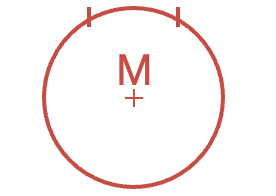
\includegraphics[width=2cm]{Legende/3 Phasen Motor.png} & \centering 3-Phasen-Motor \tabularnewline
			\hline
	\end{tabular}}
	\caption{Legende der Symbole}
	\label{tab:legende}
\end{table}